\chapter{La statistica descrittiva}
\label{cap:descrittiva}


\section*{Obiettivi di apprendimento}


\begin{multicols}{2}
\begin{tcolorbox}[width=1\linewidth, halign=left, colframe=blue!60, colback=white, boxsep=1mm, arc=3mm]

Domande

\begin{myitemize}
	\item Come posso conoscere le propriet\`a di un data frame?
	\item Come si crea ed esegue uno script in RStudio?
	\item Come si costruiscono tabelle di frequenza e contingenza?
	\item Come si calcolano misure di centralit\`a e dispersione?
	\item Come si calcola la correlazione tra due variabili numeriche?
	\item Come si costruiscono bar, mosaic, box e scatter plots e istogrammi?
\end{myitemize}

\end{tcolorbox} 
\columnbreak
\begin{tcolorbox}[width=1\linewidth, halign=left, colframe=blue!60, colback=white, boxsep=1mm, arc=3mm]

Obiettivi

\begin{myitemize}
	\item Mostrare le propriet\`a di un data frame incluso dimensioni, nome degli attributi, e prime/ultime righe 
	\item Salvare i comandi R in uno script
	\item Saper riassumere numericamente e visivamente dati categorici e numerici
	\item Saper identificare relazioni lineari tra variabili numeriche
\end{myitemize}

\end{tcolorbox} 
\columnbreak
\end{multicols}


\section{Creare uno script in RStudio}
\label{sec:Rscript}

Sino a ora ci siamo limitati a usare la console che RStudio ci mette a disposizione. Come abbiamo per\`o accennato in Sezione~\ref{sec:RStudio}, la console non offre nessuna persistenza, ovvero chiudendo RStudio perdiamo tutto il lavoro fatto. Per il resto del corso, useremo invece uno script R\footnote{In realt\`a andremo a usare anche la console per fare dei piccoli test.}, che garantisce che il nostro lavoro sia sempre disponibile assicurando cos\`i la riproducibilit\`a delle nostre analisi.


\begin{mybox}{Script R}	
	
Uno script R \`e un elenco di comandi R che viene salvato in un file che (indovinate un po' che fantasia) finisce con estensione ``.R''. Salvare i comandi in uno script \`e utile per poterli eseguire di nuovo, per esempio utilizzando la funzione \lsin{source()}

\end{mybox}


\noindent Andiamo quindi a creare un nuovo file attraverso il men\`u \lsin{File} $\rightarrow$ \lsin{New file}  $\rightarrow$ \lsin{R script}. Si apre quindi un nuovo pannello in alto a sinistra, che abbiamo gi\`a visto in Figura~\ref{fig:rstudio-script}. 
%
Usiamo ancora un momento la console per creare una cartella dove il nostro script andr\`a salvato:

\begin{lstlisting}[style=Rstyle]
filepath <- "~/Desktop/Rlab/script/"
dir.create(filepath, recursive = TRUE)
\end{lstlisting}
%
Usiamo quindi di nuovo il men\`u di RStudio per salvare il nostro script: \lsin{File} $\rightarrow$ \lsin{Save As}  $\rightarrow$ andiamo dare un nome al nostro  script (\lsin{gapminder_analysis.R}) e andiamo a scegliere la cartella che abbiamo appena creato.


\subsection{Eseguire pezzi di codice in RStudio}	

Per eseguire la linea di codice corrente (quella su cui avete il cursore) o un blocco di codice (che avrete precedentemente evidenziato) potete:

\begin{myitemize}
	\item cliccare sul bottone \lsin{Run} sul pannello dell'editor dello script (rappresentato con un'icona che mostra un documento e una freccia verde)
	\item usare uno delle diverse opzioni \lsin{Run...} nel men\`u \lsin{Code}
	\item premere \lsin{Ctrl+Return} (Windows/Linux) o \lsin{Cmd+Return} (Mac OS X)
\end{myitemize}

\section{Carichiamo ed esploriamo il dataset Gapminder}


Spostiamoci ora nel pannello dello script\footnote{Per il codice da salvare nello script, lo sfondo passa dal grigio al bianco.}, e andiamo a scrivere il codice per scaricare il dataset che useremo nel resto delle dispense, che avete di nuovo a disposizione online. Come abbiamo gi\`a fatto in Sezione~\ref{sec:data_loading}, il primo passo \`e scaricarlo in una cartella locale utilizzando la funzione \lsin{download.file()}:

\begin{lstlisting}[style=Rstylescript]
# L'indirizzo dal quale scaricare i dati
url <- "https://t.ly/LdARM"

# Il nome del file e dove salvarlo nel proprio computer
filename <- "gapminder.csv"
filepath <- "~/Desktop/Rlab/data/"

# Cambia la directory
setwd(filepath)

# Scarica il file
download.file(url, paste(filepath, filename, sep=""), mode = "w")

# Leggi il file
gapminder <- read.csv(filename)
\end{lstlisting}
%
Andiamo ad eseguire tutto questo blocco di codice evidenziandolo con il mouse e poi usando il bottone \lsin{Run} disponibile in RStudio.

\noindent Usiamo ora la console per esplorare velocemente questo dataset:


\begin{lstlisting}[style=Rstyle]
head(gapminder)
              country world_region income_group_2017
1         Afghanistan         asia        Low income
2             Albania       europe     Middle income
3             Algeria       africa     Middle income
4             Andorra       europe       High income
5              Angola       africa     Middle income
6 Antigua and Barbuda     americas       High income
  happiness_score_2011 gov_health_spending_percent
1                 38.3                        1.59
2                 58.7                        8.42
3                 53.2                        8.12
4                 <NA>                       21.30
5                 55.9                        7.18
6                 <NA>                       16.70
\end{lstlisting}


\begin{lstlisting}[style=Rstyle]
tail(gapminder)
      country world_region income_group_2017
184   Vanuatu         asia     Middle income
185 Venezuela     americas     Middle income
186   Vietnam         asia     Middle income
187     Yemen         asia     Middle income
188    Zambia       africa     Middle income
189  Zimbabwe       africa        Low income
    happiness_score_2011 gov_health_spending_percent
184                   NA                       18.20
185                 65.8                        7.52
186                 57.7                        7.79
187                 37.5                        4.33
188                 50.0                       15.60
189                 48.5                          NA
\end{lstlisting}
%
Da questo ultimo comando, scopriamo che il nostro data frame ha \lsin{193} righe, anche se possiamo vederlo in modo diverso:

\begin{lstlisting}[style=Rstylescript]
nrow(gapminder)
ncol(gapminder)
dim(gapminder)
\end{lstlisting}
%	
quando eseguiamo questo codice, otteniamo il seguente output:

\begin{lstlisting}[style=Rstyle]
[1] 189
[1] 5
[1] 189   5
\end{lstlisting}
%
la \textbf{numerosit\`a} del nostro "campione" \`e \lsin{189}, e il numero di attributi (dati che abbiamo raccolto) che lo descrive \`e \lsin{5}. Per conoscere il nome di tali attributi possiamo usare il seguente comando:


\begin{lstlisting}[style=Rstylescript]
colnames(gapminder)
\end{lstlisting}

\begin{lstlisting}[style=Rstyle]
[1] "country"                     "world_region"
[3] "income_group_2017"           "happiness_score_2011"
[5] "gov_health_spending_percent"
\end{lstlisting}


\section{I dati categorici}

\subsection{Tabelle di frequenza}

Per creare \textbf{tabelle di frequenza assoluta} usiamo la funzione \lsin{table()}:

\begin{lstlisting}[style=Rstylescript]
freq_a <- table(gapminder$world_region)
\end{lstlisting}

\begin{lstlisting}[style=Rstyle]
freq_a	
 africa americas     asia   europe 
     53       34       57       45 
\end{lstlisting}
%
Notiamo che le modalit\`a della nostra variabile categorica sono ordinate in ordine alfabetico.

\noindent Per ottenere le \textbf{frequenze relative} a partire da quelle assolute usiamo la funzione \lsin{prop.table()}:

\begin{lstlisting}[style=Rstylescript]
freq_r <- prop.table(freq_a)
\end{lstlisting}

\begin{lstlisting}[style=Rstyle]
freq_r	
   africa  americas      asia    europe 
0.2804233 0.1798942 0.3015873 0.2380952
\end{lstlisting}
%
andiamo ora trasformarli in percentuale e renderli un po' pi\`u leggibili:

\begin{lstlisting}[style=Rstylescript]
freq_r <- freq_r*100
freq_r <- round(freq_r, 1)
\end{lstlisting}


\begin{lstlisting}[style=Rstyle]
freq_r	
 africa americas     asia   europe 
   28.0     18.0     30.2     23.8
\end{lstlisting}

\vspace{0.5cm} 

\begin{exercise}\label{ex4.1}
	
\noindent Scrivere il codice per calcolare la frequenza assoluta e relativa dell'attributo \lsin{income_group_2017}.	
 
\noindent Qual \`e la \textbf{moda} di questa variabile?

\end{exercise}

\subsection{Bar plot}

\noindent Andiamo ora a crearne il bar plot utilizzando la libreria R \lsin{ggplot2}, che \`e la libreria R pi\`u usata per creare dei grafici\footnote{R include anche un pacchetto base per la grafica che offre comunque dei risultati molto professionali. \lsin{ggplot2} \`e tuttavia molto pi\`u versatile a causa dell'ecosistema che lo supporta.}. Per utilizzarla dobbiamo innanzitutto caricarla (vedi Sezione~\ref{sec:R_package}):

\begin{lstlisting}[style=Rstylescript]
library(ggplot2)
\end{lstlisting}
%
\lsin{ggplot2} richiede, nella sua versione pi\`u semplice, il data frame dove sono salvati i dati da visualizzare, quali variabili devono essere visualizzate e in quali assi e il tipo di grafico che si vuole utilizzate:

\begin{lstlisting}[style=Rstylescript]
ggplot(gapminder, aes(x=world_region)) + geom_bar()
\end{lstlisting}
% 
\lsin{geom_bar()} indica che vogliamo costruire un bar plot. Il comportamento di default di questa funzione \`e andare a contare quanti valori ci sono per ciascuna modalit\`a, per andare a calcolare l'altezza della barra. Prende diversi argomenti quali la dimensione della barra, il suo colore e quello del suo bordo:

\begin{lstlisting}[style=Rstylescript]
ggplot(gapminder, aes(x=world_region)) + geom_bar(width=0.8, fill="gray", colour="black")
\end{lstlisting}
%
Possiamo anche andare a cambiare le etichette degli assi e ad aggiungere un titolo e sottotitolo:

\begin{lstlisting}[style=Rstylescript]
ggplot(gapminder, aes(x=world_region)) + geom_bar(width=0.8, fill="gray", colour="black") + xlab("") + ylab("Count") + ggtitle("World Region", subtitle="Gapminder data")
\end{lstlisting}
%
Infine, possiamo passare a uno sfondo bianco, per migliorare la leggibilit\a`, come mostrato in Figura~\ref{fig:barplot}:

\begin{lstlisting}[style=Rstylescript]
ggplot(gapminder, aes(x=world_region)) + geom_bar(width=0.8, fill="gray", colour="black") + xlab("") + ylab("Count") + ggtitle("World Region", subtitle="Gapminder data") + theme_bw()
\end{lstlisting}
%
In ciascuna di queste operazioni, \lsin{ggplot2} va a creare un \lsin{layer} per ogni nuovo elemento\footnote{Troverete questa informazione utile se mai dovreste andare a debuggare un grafico creato con  \lsin{ggplot2}.}.

\noindent Andiamo ora ad assegnare il nostro grafico a una variabile\footnote{Anche i grafici sono variabili.}:

\begin{lstlisting}[style=Rstylescript]
barplot <- ggplot(gapminder, aes(x=world_region)) + geom_bar(width=0.8, fill="gray", colour="black") + xlab("") + ylab("Count") + ggtitle("World Region", subtitle="Gapminder data") + theme_bw()
\end{lstlisting}

\begin{figure}[h]
 \centering
  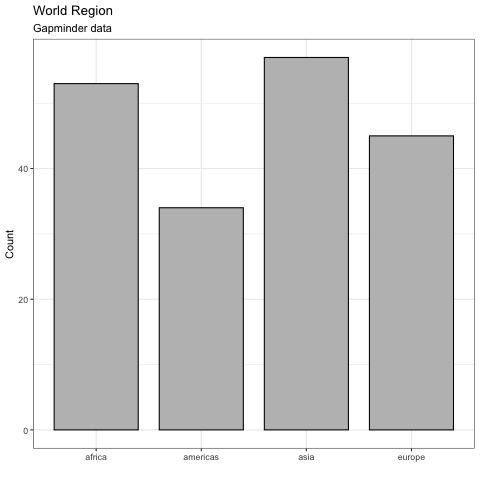
\includegraphics[width=0.75\textwidth]{images/bar_plot.png}
  \label{fig:barplot}
 \caption{Bar plot. Rappresentazione grafica di una variabile categorica. Ciascuna modalit\`a viene rappresentata da una barra, la cui dimensione \`e proporzionale alla sua frequenza, in questo caso assoluta.}
\end{figure}


\subsection{Relazione tra due variabili categoriche}

La funzione \lsin{table()} pu\`o anche essere usata per costruire \textbf{tabelle di contingenza}:

\begin{lstlisting}[style=Rstylescript]
tab_cont <- table(gapminder$world_region, gapminder$income_group_2017)
\end{lstlisting}

\begin{lstlisting}[style=Rstyle]
tab_cont	
         High income Low income Middle income
africa             1         27            25
americas           8          1            25
asia              15          2            40
europe            30          0            15
\end{lstlisting}
%
Notiamo che, di nuovo, le variabili sono ordinate in ordine alfabetico. La tabella sarebbe per\`o di pi\`u facile interpretazione se le colonne fossero ordinate da low a high income:

\begin{lstlisting}[style=Rstylescript]
ord <- c(2, 3, 1) 
tab_cont <- tab_cont[, ord]
\end{lstlisting}

\begin{lstlisting}[style=Rstyle]
tab_cont
           Low income Middle income High income
  africa           27            25           1
  americas          1            25           8
  asia              2            40          15
  europe            0            15          30
\end{lstlisting}
%
Questa tabella di contingenza mostra le frequenze assolute. Per ottenere le frequenze relative a partire da quelle assolute usiamo di nuovo la funzione \lsin{prop.table()}:

\begin{lstlisting}[style=Rstylescript]
tab_cont_rel <- prop.table(tab_cont)
\end{lstlisting}
%
senza nessun argomento, ci ritorna la frequenza relativa di ciascuna coppia di modalit\`a nel dataset, e come tale, somma a 1:


\begin{lstlisting}[style=Rstyle]
tab_cont_rel
            Low income Middle income High income
  africa   0.142857143   0.132275132 0.005291005
  americas 0.005291005   0.132275132 0.042328042
  asia     0.010582011   0.211640212 0.079365079
  europe   0.000000000   0.079365079 0.158730159
  
sum(tab_cont_rel)
[1] 1
\end{lstlisting}
%
Per creare le frequenze relative per righe o per colonne, si usa il parametro \lsin{margin}, che prende il valore \lsin{1} per le righe e \lsin{2} per le colonne:

\begin{lstlisting}[style=Rstylescript]
tab_cont_rel_row <- prop.table(tab_cont, margin=1)
tab_cont_rel_col <- prop.table(tab_cont, margin=2)
\end{lstlisting}


\begin{lstlisting}[style=Rstyle]
tab_cont_rel_row
         Low income Middle income High income
africa   0.50943396    0.47169811  0.01886792
americas 0.02941176    0.73529412  0.23529412
asia     0.03508772    0.70175439  0.26315789
europe   0.00000000    0.33333333  0.66666667

tab_cont_rel_col
         Low income Middle income High income
africa   0.90000000    0.23809524  0.01851852
americas 0.03333333    0.23809524  0.14814815
asia     0.06666667    0.38095238  0.27777778
europe   0.00000000    0.14285714  0.55555556
\end{lstlisting}


\vspace{0.5cm} 

\begin{exercise}\label{ex4.2}
	
\noindent Scrivere il codice per trasformare la frequenza relativa contenuta in \lsin{tab_cont_rel_col} in percentuale, con una sola cifra decimale.

\noindent Per ciascuna classe di income, qual \`e la regione del mondo con la frequenza pi\`u alta?

\end{exercise}


\subsection{Mosaic plot}

Le tabelle di contingenza possono essere visualizzate come \textbf{Mosaic plot} usando la funzione \lsin{mosaicplot()}:

\begin{lstlisting}[style=Rstylescript]
mosaicplot(tab_cont)
\end{lstlisting}
%
Possiamo renderlo pi\`u chiaro usando i colori (anche a costo di aggiungere informazione ridondante):

\begin{lstlisting}[style=Rstylescript]
mosaicplot(tab_cont, color = c("darkgreen", "gray70", "darkmagenta"))
\end{lstlisting}
%
e le etichette per assi e titolo, ottenendo il grafico mostrato in Figura~\ref{fig:mosaic}:

\begin{lstlisting}[style=Rstylescript]
mosaicplot(tab_cont, color = c("darkgreen", "gray70", "darkmagenta"), xlab ="World Region", ylab = "Income group", main="Income group by world region")
\end{lstlisting}


\begin{figure}[h]
 \centering
  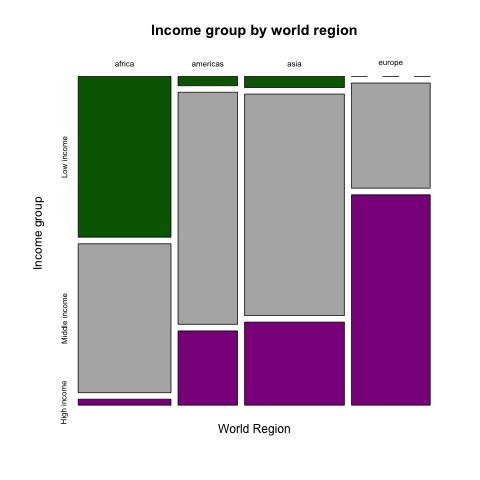
\includegraphics[width=0.75\textwidth]{images/mosaic_plot.png}
  \label{fig:mosaic}
 \caption{Mosaic plot. Rappresentazione grafica della relazione tra due variabili categoriche: world region (sull'asse delle ascisse) e income group (sull'asse delle ordinate). I rettangoli sono colorati in base all'income group, con verde, grigio e viola a indicare alto, medio e basso income, rispettivamente. Ogni rettangolo mostra la percentuale di osservazioni per ciascuna coppia di modalit\`a delle due variabili. La linea tratteggiata indica che non \`e presente nessuna osservazione per l'intersezione di due modalit\`a (paesi europei con low income).}
\end{figure}

\section{I dati numerici}

\subsection{Misure di centralit\`a e dispersione}
\label{sec:centdisp}

R offre delle funzioni per calcolare diverse misure sia di  centralit\`a sia di dispersione. Per la \textbf{media} e la \textbf{deviazione standard} usiamo:

\begin{lstlisting}[style=Rstylescript]
mean_happiness <- mean(gapminder$happiness_score_2011)
sd_happiness <- sd(gapminder$happiness_score_2011)
\end{lstlisting}

\begin{lstlisting}[style=Rstyle]
mean_happiness
[1] NA

sd_happiness
[1] NA
\end{lstlisting}
%
cosa \`e successo? Se ci sono dei valori a \lsin{NA}, R ritorner\`a \lsin{NA}. Come facciamo ad escluderli? Con il parametro \lsin{na.rm}:

\begin{lstlisting}[style=Rstylescript]
mean_happiness <- mean(gapminder$happiness_score_2011, na.rm=TRUE)
sd_happiness <- sd(gapminder$happiness_score_2011, na.rm=TRUE)
\end{lstlisting}

\begin{lstlisting}[style=Rstyle]
mean_happiness
[1] 54.05252

sd_happiness
[1] 10.81201
\end{lstlisting}
%
Calcoliamo ora \textbf{mediana} e \textbf{quartili}, \textbf{massimo} e \textbf{minimo}:

\begin{lstlisting}[style=Rstylescript]
median_happiness <- median(gapminder$happiness_score_2011, na.rm=TRUE)
quartile_happiness <- quantile(gapminder$happiness_score_2011, na.rm=TRUE)

min_happiness <- min(gapminder$happiness_score_2011, na.rm=TRUE)
max_happiness <- max(gapminder$happiness_score_2011, na.rm=TRUE)
\end{lstlisting}

\begin{lstlisting}[style=Rstyle]
median_happiness
[1] 52.3

quartile_happiness
   0%   25%   50%   75%  100%
29.40 46.75 52.30 62.85 77.90

min_happiness
[1] 29.4

max_happiness
[1] 77.9
\end{lstlisting}


\vspace{0.5cm} 

\begin{exercise}\label{ex4.3}
	
\noindent Scrivere il codice per calcolare range e range interquartile.

\noindent Secondo voi, alla luce di tutte le statistiche calcolate, che forma ha questa distribuzione?

\end{exercise}

\subsection{Istogrammi}
\label{sec:histo}

Andiamo ora a costruirne l'\textbf{istogramma}, di nuovo passo passo:

\begin{lstlisting}[style=Rstylescript]
ggplot(gapminder, aes(x=happiness_score_2011)) + geom_histogram()
\end{lstlisting}

\begin{lstlisting}[style=Rstyle]
`stat_bin()` using `bins = 30`. Pick better value
with `binwidth`.
(*@\textbf{\textcolor{red}{Warning message: }}@*)
Removed 50 rows containing non-finite outside the
scale range (`stat_bin()`).
\end{lstlisting}
%
questo messaggio ci sta dando numerose informazioni: \emph{(i)} \lsin{ggplot} sta creando 30 gruppi (bins, corrispondenti a 30 barre), andando a dividere i vostri dati equamente in questi bins e \emph{(ii)} 50 righe del vostro dataset sono state eliminate perch\`e non hanno un valore finito. Cosa possono essere questi valori non finiti? 

\noindent Se avete risposto \lsin{NA}, avete ragione. Andiamo a verificarlo:

\begin{lstlisting}[style=Rstyle]
is.na(gapminder$happiness_score_2011)
  [1] FALSE FALSE FALSE  TRUE FALSE  TRUE FALSE FALSE
  [9] FALSE FALSE FALSE  TRUE FALSE FALSE  TRUE FALSE
 [17] FALSE  TRUE FALSE  TRUE FALSE FALSE FALSE FALSE
 [25]  TRUE FALSE FALSE FALSE FALSE FALSE FALSE  TRUE
 [33] FALSE FALSE FALSE FALSE FALSE FALSE FALSE FALSE
 [41] FALSE  TRUE FALSE  TRUE FALSE FALSE FALSE FALSE
 [49]  TRUE FALSE FALSE FALSE FALSE  TRUE  TRUE FALSE
 [57]  TRUE  TRUE FALSE FALSE FALSE  TRUE FALSE FALSE
 [65] FALSE FALSE  TRUE FALSE FALSE  TRUE  TRUE FALSE
 [73] FALSE FALSE FALSE  TRUE FALSE FALSE FALSE FALSE
 [81] FALSE FALSE FALSE FALSE FALSE FALSE FALSE FALSE
 [89]  TRUE FALSE FALSE FALSE FALSE FALSE FALSE  TRUE
 [97]  TRUE FALSE FALSE FALSE FALSE FALSE  TRUE FALSE
[105] FALSE  TRUE FALSE FALSE FALSE  TRUE FALSE  TRUE
[113] FALSE FALSE FALSE FALSE  TRUE  TRUE  TRUE FALSE
[121] FALSE FALSE FALSE FALSE  TRUE  TRUE FALSE FALSE
[129]  TRUE FALSE FALSE  TRUE FALSE FALSE FALSE FALSE
[137] FALSE FALSE FALSE FALSE FALSE  TRUE  TRUE  TRUE
[145] FALSE FALSE FALSE  TRUE FALSE FALSE FALSE FALSE
[153]  TRUE  TRUE FALSE FALSE  TRUE FALSE FALSE  TRUE
[161]  TRUE  TRUE FALSE  TRUE FALSE  TRUE FALSE FALSE
[169] FALSE FALSE FALSE  TRUE FALSE  TRUE FALSE FALSE
[177] FALSE FALSE  TRUE FALSE FALSE FALSE FALSE  TRUE
[185] FALSE FALSE FALSE FALSE FALSE
\end{lstlisting}
%
Se state pensando di contare quanti \lsin{TRUE} ci sono, sappiate che \lsin{TRUE} equivale a \lsin{1} in R, e che \lsin{FALSE} equivale a \lsin{0}. Quindi possiamo sommare tutti i \lsin{TRUE} con la funzione \lsin{sum()}:

\begin{lstlisting}[style=Rstyle]
num_na <- is.na(gapminder$happiness_score_2011)
sum(num_na)
[1] 50
\end{lstlisting}
%
\lsin{ggplot} ha effettivamente scartato i valori a \lsin{NA}.

\noindent Ignoriamo perci\`o questo warning e andiamo ora a lavorare sul numero di bins, usando il parametro \lsin{binwidth}, come suggerito da R, e nel migliorarne la grafica, con gli stessi parametri che abbiamo visto per il bar plot:

\begin{lstlisting}[style=Rstylescript]
ggplot(gapminder, aes(x=happiness_score_2011)) + geom_histogram(binwidth=5, width=0.8, fill="gray", color="black")
\end{lstlisting}
%
Sistemiamo ora labels, titolo e sfondo, ottenendo il grafico in Figura~\ref{fig:histogram} e assegniamolo a una variabile:

\begin{lstlisting}[style=Rstylescript]
histogram_happiness <- ggplot(gapminder, aes(x=happiness_score_2011)) + geom_histogram(binwidth=5, width=0.8, fill="gray", color="black") + xlab("Score") + ylab("Counts") + ggtitle("World happiness in 2011", subtitle="Gapminder data") + theme_bw()
\end{lstlisting}


\begin{figure}[h]
 \centering
  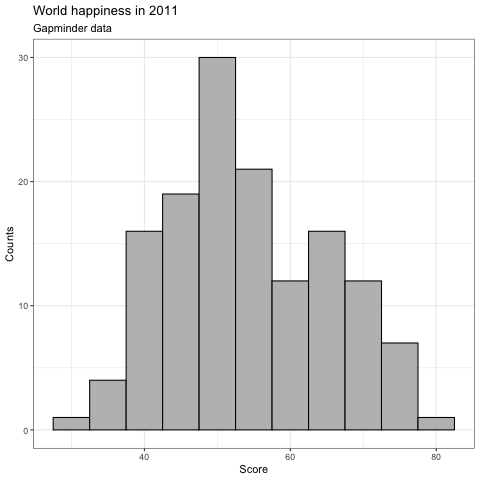
\includegraphics[width=0.75\textwidth]{images/histogram.png}
  \label{fig:histogram}
 \caption{Istogramma. Rappresentazione grafica di una variabile numerica. La variabile subisce un processo di Discretizzazione, che identifica un certo numero di classi, ognuna rappresentata da una barra, la cui dimensione \`e proporzionale alla sua frequenza, in questo caso assoluta.}
\end{figure}

\vspace{0.5cm} 

\begin{exercise}\label{ex4.4}
	
\noindent Scrivere il codice per calcolare tutte le statistiche descritte in precedenza per l'attributo \lsin{gov_health_spending_percent}.

\noindent Costruirne poi l'istogramma, colorando le barre di bianco con dei bordi rossi.

\end{exercise}

\subsubsection{Box plot}
\label{sec:boxplot}

Visualizziamo ora coma si distribuisce il livello di felicit\`a a seconda dell'income group usando un \textbf{boxplot}:

\begin{lstlisting}[style=Rstylescript]
ggplot(gapminder, aes(x=happiness_score_2011, y=income_group_2017)) + geom_boxplot()
\end{lstlisting}

\begin{lstlisting}[style=Rstyle]
(*@\textbf{\textcolor{red}{Warning message: }}@*)
Removed 50 rows containing non-finite outside the
scale range (`stat_boxplot()`).
\end{lstlisting}
%
anche questa volta l'income group viene visualizzato in ordine alfabetico, ma andarne a cambiare l'ordine \`e un po' pi\`u complesso di quello che abbiamo fatto per il mosaic plot. Infatti, \lsin{ggplot2} trasforma i dati categorici in \lsin{factor}, un tipo di dato che non avevamo ancora introdotto. Vediamoli adesso:

\begin{lstlisting}[style=Rstyle]
income_group <- gapminder$income_group_2017

class(income_group)
[1] "character"

income_group <- as.factor(income_group)

class(income_group)
[1] "factor"

head(income_group)
[1] Low income    Middle income Middle income
[4] High income   Middle income High income   
Levels: High income Low income Middle income
\end{lstlisting}
%
quello che vogliamo andare a riordinare sono i livelli:

\begin{lstlisting}[style=Rstylescript]
gapminder$income_group_2017 <- factor(gapminder$income_group_2017, levels=c("Low income", "Middle income", "High income"))	
\end{lstlisting}

\begin{lstlisting}[style=Rstyle]
head(gapminder$income_group_2017)
[1] Low income    Middle income Middle income
[4] High income   Middle income High income  
Levels: Low income Middle income High income
\end{lstlisting}
%
Torniamo quindi al nostro boxplot:

\begin{lstlisting}[style=Rstylescript]
ggplot(gapminder, aes(x=happiness_score_2011, y=income_group_2017)) + geom_boxplot()
\end{lstlisting}
%
I gruppi sono ora ordinati. Miglioriamone ora la grafica, ottenendo il grafico mostrato in Figura~\ref{fig:boxplot}:


\begin{lstlisting}[style=Rstylescript]
boxplot <- ggplot(gapminder, aes(x=happiness_score_2011, y=income_group_2017)) + geom_boxplot(fill="grey") + xlab("Score") + ylab("") + ggtitle("World happiness by income group", subtitle="Gapminder data") + theme_bw()
\end{lstlisting}

\begin{figure}[h]
 \centering
  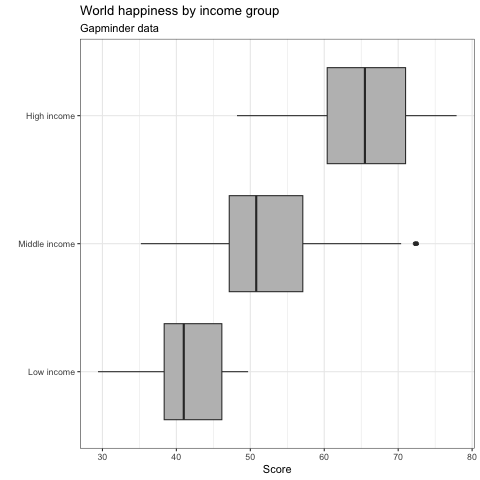
\includegraphics[width=0.75\textwidth]{images/boxplot.png}
  \label{fig:boxplot}
 \caption{Boxplot. Rappresentazione grafica congiunta di una variabile numerica e una variabile categorica. La variabile numerica viene rappresentata utilizzando, in questo caso, tre diversi boxplot, uno per ciascuna variabile categorica. Questo ci permette di confrontare le tre distribuzioni.}
\end{figure}


\vspace{0.5cm} 

\begin{exercise}\label{ex4.5}
	
\noindent Scrivere il codice per costruire il boxplot che mostra le differenze in happiness score a seconda delle world region.

\noindent In quale regione le persone sono meno felici? \\

\noindent \textbf{Difficolt\`a elevata:} Qual \`e l'happiness score medio in ogni regione? 


	\exnote{Suggerimenti}%
	\begin{myitemize}
		\item Per calcolare l'happiness score medio, dovete estrarre solo la porzione di dati che appartiene a una data regione.
	\end{myitemize}

\end{exercise}


\section{La relazione tra due variabili numeriche}

Andiamo ora a utilizzare il \textbf{coefficiente di Pearson} per calcolare la \textbf{correlazione} tra happiness score e health spending:

\begin{lstlisting}[style=Rstylescript]
cr <- cor(x=gapminder$gov_health_spending_percent, y=gapminder$happiness_score_2011)
\end{lstlisting}

\begin{lstlisting}[style=Rstyle]
[1] NA
\end{lstlisting}
%
Abbiamo di nuovo il problema con gli \lsin{NA}, usiamo il manuale per risolverlo:

\begin{lstlisting}[style=Rstyle]
?cor
\end{lstlisting}

\begin{lstlisting}[style=Rstylescript]
cr <- cor(x=gapminder$gov_health_spending_percent, y=gapminder$happiness_score_2011, use="complete.obs")
\end{lstlisting}

\begin{lstlisting}[style=Rstyle]
[1] 0.3985756
\end{lstlisting}

\subsection{Scatter plot}

\begin{figure}[h]
 \centering
  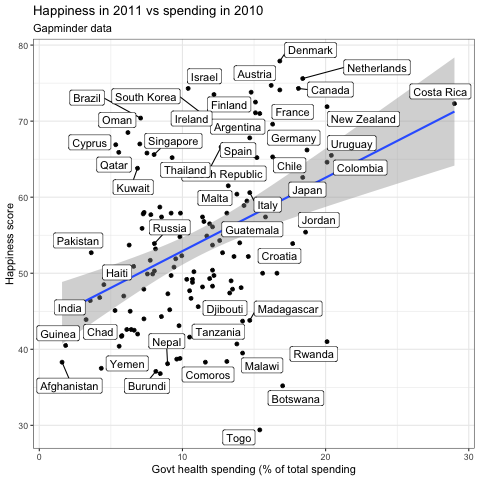
\includegraphics[width=0.75\textwidth]{images/scatter.png}
  \label{fig:scatter}
 \caption{Scatter plot. Rappresentazione grafica della relazione tra due variabili numeriche. Ciascun asse mostra una delle due variabili, la linea di tendenza (in blu) viene mostrata insieme al suo intervallo di confidenza.}
\end{figure}

Visualizziamo ora la relazione tra l'happiness score e lo spending percentage usando uno \textbf{scatterplot}:

\begin{lstlisting}[style=Rstylescript]
ggplot(gapminder, aes(x=gov_health_spending_percent, y=happiness_score_2011)) + geom_point() 
\end{lstlisting}

\begin{lstlisting}[style=Rstyle]
(*@\textbf{\textcolor{red}{Warning message: }}@*)
Removed 57 rows containing missing values or values outside the scale range (`geom_point()`).
\end{lstlisting}
%
Perch\'e ora ci sono 57 valori a \lsin{NA}?

\begin{lstlisting}[style=Rstylescript]
scatter <- ggplot(gapminder, aes(x=gov_health_spending_percent, y=happiness_score_2011)) + geom_point() + xlab("Govt health spending (% of total spending") + ylab("Happiness score") + ggtitle("Happiness in 2011 vs spending in 2010", subtitle="Gapminder data") + theme_bw()
\end{lstlisting}
%
Andiamo per ultimo ad aggiungere una linea di tendenza:

\begin{lstlisting}[style=Rstylescript]
scatter <- scatter + geom_smooth(method="lm")
\end{lstlisting}
%
Possiamo anche mettere un'etichetta per mostrare alcuni dei paesi, come mostrato in Figura~\ref{fig:scatter}, usando il pacchetto R \lsin{ggrepel} (che avete installato durante l'Esercizio 2.5, Sezione~\ref{sec:R_package}):

\begin{lstlisting}[style=Rstylescript]
library(ggrepel)
scatter <- scatter + geom_label_repel(aes(label = country)
\end{lstlisting}




\vspace{0.5cm}

\begin{tcolorbox}[width=1\linewidth, halign=left, colframe=blue!60, colback=white, boxsep=1mm, arc=3mm]

\textbf{Punti principali}

\begin{myitemize}
    \item Usare \lsin{nrow(), ncol(), dim(), colnames(), head()} e \lsin{tail()} per esplorare la struttura di un data frame 
    \item Usare \lsin{table()} e \lsin{prop.table()} per calcolare frequenze assolute e relative
	\item Usare \lsin{mean(), sd(), median(), quantile(), min()} e \lsin{max()} per calcolare le corrispondenti misure di centralit\`a e dispersione
    \item Usare la funzione \lsin{is.na()} e il parametro \lsin{na.rm} per gestire i valori a \lsin{NA}
    \item Usare \lsin{cor} per calcolare la correlazione tra due variabili numeriche
    \item Usare il pacchetto R \lsin{ggplot2} per visualizzare i dati
\end{myitemize}

\end{tcolorbox}
